% Dossier de gestion de la documentation
% Version 1.2

% Historique des versions
% 19/01/08 1.0 Création et remplissage (Mikado)
% 20/01/08 1.1 Entrée en phase de finalisation (Mikado)
% 21/01/08 1.2 Finalisation du document (Mikado)

\renewcommand\docname{DGDv1.2}
\renewcommand\docauthor{Fabrice GABOLDE}
\renewcommand\docstatus{LIVRABLE}
\part{Dossier de gestion de la documentation}

\label{part:dgd}

\chapter{Introduction}

\section*{Document \docname{}}

Auteur : \docauthor{}

Etat : \docstatus{}

\section{Présentation du projet}

Il existe aujourd'hui de nombreux sites isolés et/ou difficiles d'accès qui nécessitent une surveillance et parfois des actions à distance. Ces sites se situent dans des espaces très différents tels que les citernes placées dans les forêts escarpées du pourtour méditerranéen, les réservoirs utilisés pour l'autonomie des chantiers dans le grand Nord mais aussi les personnes âgées qui se retrouvent souvent isolées.

Actuellement tous les contrôles et actions sont réalisés par un opérateur qui doit se déplacer sur le site. Il n'y a donc que très peu de réactivité, on ne peut pas avoir un suivi fin des évolutions et des problèmes graves (par exemple la fuite d'un réservoir) ne peuvent pas être traités rapidement.

\paragraph{Etude COPEVUE}
L'objet de l'étude est la mise en place d'un système générique de surveillance et d'action à distance sur des sites isolés. Le système devra être évolutif, autonome et fiable.

\section{Présentation du document}

Ce document (Dossier de gestion de la documentation) présente les différentes normes et suggestions applicables à la production de documents dans le cadre du projet COPEVUE. Le but de ce document est de fournir une base pour assurer la qualité du projet dans son ensemble.

\subsection{Objectifs}

Voici les objectifs de ce document :
\begin{itemize}
\item Présentation des documents à produire
\item Présentation des règles de production
\item Définition du cycle de vie, états et version d'un document
\item Présentation de la gestion des documents produits
\item Présentation de la gestion des fichiers et dossiers
\item Présentation de la gestion de la communication interne
\end{itemize}

\section{Documents applicables et de référence}

\subsection{Documents applicables}

\begin{itemize}
\item Dossier de gestion de la documentation (DGD), ce document
\end{itemize}

\subsection{Documents de référence}

Aucun.

\chapter{Règles générales}

\section{Identification des documents}

Les documents seront identifiés par une abréviation standard et leur numéro de version (exem\-ple pour ce dossier de gestion de la documentation : \docname). Le numéro de version sera incrémenté à chaque contribution au document.

\section{Norme de présentation}

Les documents présenteront le même style et la même page de garde (aux informations propres à chaque document près : titre, version, etc.) dans un but d'uniformisation.
Voir \fullref{chapter:modeles_documents} pour les modèles de documents utilisés.

\section{Etats d'un document}

Un document doit à tout moment être parmi l'un de ces états (voir figure \fullref{figure:dossier_gestion_documentation_etats_documents}) :
\begin{description}
\item[En cours]{Le document est en cours de rédaction par son (ou ses) auteur(s), et n'est pas encore présentable ni même vérifié. L'option \verb|draft| doit être présente dans les options globales du document.}
\item[Attente]{Le document est en attente de vérification par le CdP, sa rédaction est arrêtée ; il peut repasser \textbf{en cours} si le CdP a des remarques à faire concernant le contenu. L'option \verb|draft| doit être présente dans les options globales du document.}
\item[Validé]{Le document a été validé pour son contenu par le CdP ; il peut repasser \textbf{en cours} si le RQ a des remarques à faire concernant la conformité. L'option \verb|draft| doit être présente dans les options globales du document.}
\item[Livrable]{Le document a été validé pour sa conformité par le RQ. L'option \verb|draft| doit être remplacée dans les options globales du document par l'option \verb|final|.}
\end{description}

\begin{figure}[!htp]
\begin{center}
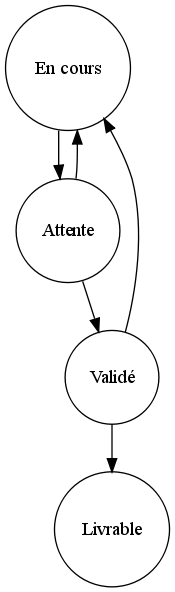
\includegraphics[width=0.15\textwidth]{qualite_dossier_gestion_documentation_etats_documents.png}
\caption{Etats d'un document}
\label{figure:dossier_gestion_documentation_etats_documents}
\end{center}
\end{figure}

\section{Cycle de vie d'un document}

\subsection{Production du document}

L'auteur principal du document est le collaborateur, ou le groupe de collaborateur, désigné par le CdP pour travailler dessus en priorité. Les autres membres du groupe de travail peuvent ensuite participer à la production du document si nécessaire. L'auteur principal doit commencer la production du document en mettant en place le template \LaTeX{} fourni pour ce type de document et le plan général du document. Il peut pour ce faire s'aider des plans types (voir \fullref{chapter:plans_types}).

\subsection{Vérification et validation du document}

La vérification du document se fait en deux étapes : d'abord, le CdP vérifie le contenu du document. Il peut à ce stade le renvoyer à l'auteur principal si des problèmes ont été relevés. Puis, le RQ vérifie la conformité du document. De même, il peut à ce stade le renvoyer à l'auteur principal en cas de non-conformité trop importante.

\subsection{Archivage du document}

L'archivage du document est géré par le système de contrôle de version employé. A tout moment, sur le serveur SVN maintenu par le groupe de travail, on peut retrouver la dernière version de tout document produit, ou l'une des versions précédentes.

\section{Gestion des versions}

La numérotation des versions se fait en \verb|major.minor| et suit les règles suivantes :
\begin{itemize}
\item A la création, le numéro de version est 1.0
\item Chaque modification non-triviale (exemple de modification triviale : correction d'une ou deux fautes d'orthographe) entraîne une incrémentation du numéro mineur de version
\item Chaque modification de grande envergure (exemple de modification de grande envergure : modification du plan, changement radical du contenu \ldots) entraîne une incrémentation du numéro majeur de version et une remise à zéro du numéro mineur de version
\end{itemize}

\chapter{Gestion de la documentation produite}

\section{Documents applicables et de référence}

\subsection{Documents applicables}

Un document applicable contient des indications qui doivent être suivies à la lettre pour assurer la qualité de la production des documents qui le référencent. Un document qui référence un document applicable, mais ne le respecte pas, n'est pas validable par le responsable qualité. Par exemple :
\begin{itemize}
\item Modèle de document livrable
\item Modèle de revue de document par le responsable qualité
\item \ldots
\end{itemize}

\subsection{Documents de référence}

Un document de référence contient des indications qui n'ont pas besoin d'être suivies à la lettre, mais qui peuvent aider à la production des documents qui le référencent. Un document qui référence un document de référence, mais qui ne le respecte pas, peut tout de même être validable par le responsable qualité. Les plans types (voir \fullref{chapter:plans_types}) entrent dans la catégorie des documents de référence.

\section{Gestion physique des fichiers contenant les documents}

\subsection{Répertoires}

Chaque document produit sera placé dans son propre répertoire. Le nom du répertoire utilisé sera celui de l'abréviation du document (voir le glossaire pour les abréviations), par exemple DGD pour le dossier de gestion de la documentation. Les dossiers relatifs à la qualité seront de plus situés dans le répertoire \url{qualite/}, et ceux relatifs au travail du CdP dans le répertoire \url{cdp/}. Les images utilisées pour chaque document seront dans leur propre sous-répertoire \url{images/}, par exemple pour les images du DGD : \url{qualite/dgd/images/}.

\subsection{Procédures de sauvegarde et archivage}

Les procédures de sauvegarde et d'archivage sont celles permises par l'utilisation normale du système de contrôle de version SVN.

\chapter{Communication interne}

Le groupe de travail utilisera un certain nombre de moyens de communication en interne :
\begin{description}
\item[Réunions IRL]{Des réunions en personne auront lieu tant pendant les horaires de TP prévus par le programme qu'en dehors, en fonction des nécessités des collaborateurs et du planning du CdP.}
\item[e-mail]{Tous les membres du groupe de travail disposent d'une adresse e-mail qui a été communiquée au reste du groupe au début du projet. L'envoi d'e-mails peut servir, d'une part entre collaborateurs pour s'échanger de grandes quantités de données qui n'auraient pas lieu d'être présentes sur le serveur SVN, d'autre part au CdP pour coordonner son équipe.}
\item[IM]{Tous les membres du groupe de travail disposent d'une adresse liée à un protocole de messagerie instantanée pour assurer la communication à distance via Internet, tant en temps réel qu'en asynchrone.}
\item[SVN]{L'utilisation de SVN permet de laisser des commentaires à chaque remontée de contenu, et donc d'informer le reste de l'équipe sur ce qui a été modifié.}
\end{description}